%\documentclass[runningheads]{llncs}
\documentclass[]{llncs}
\usepackage{makeidx}
\usepackage{graphicx}
\begin{document}
\addtocmark{Southern Methodist University} % additional mark in the TOC

\title{LABORATORY EARTHQUAKE ANALYSIS}
%\subtitle{Optional Subtitle Goes Here}

\author{Olha Tanyuk\inst{1}, Daniel Davieau\inst{1}, Dr. Michael L. Blanpied\inst{2}, Dr. Charles South\inst{1} \and Dr. Daniel W. Engels\inst1}

\institute{Southern Methodist University, Dallas TX 75205, USA \and United States Geological Survey, Fort Worth, TX 76115}

\maketitle
%Problem sentence
%Motivation Sentence
%2=3 what you did to solve the problem
%1 sentence main result(singular with a number)
%1 sentence main conclusion (singular)

\begin{abstract}
In 2017 the Los Alamos National Laboratory (LANL) conducted an experiment which predicted the remaining time before {\em laboratory} earthquakes occured with 90 percent accuracy\cite{Bertrand}. LANL has since collected additional data with considerably more a-periodic laboratory earthquake failures and made it available to the public in 2019.

Given the considerably more a-periodic data can we more accurately determine when laboratory earthquakes will occur?

In this {\em new} study we apply machine learning to analyze patterns in the public LANL data. We design statistical models to predict the remaining time before laboratory earthquakes occur.  We compare predicted versus actual time remaining to determine our accuracy.\par

The result proves that impending laboratory earthquakes can be predicted with {\em(temporary 0.5680)} Mean Absolute Error. The predictions are based solely on the characteristics of recorded acoustical signals; they are not based on time intervals between prior laboratory earthquakes.\par



\end{abstract}
\section{INTRODUCTION}
%1 Paragraph Motivtion (Sets General problem domain)
Earthquakes were traditionally predicted based on the recurrence interval of past earthquakes. Because earthquake recurrence is not constant for a given fault, predictions can only be made within broad time windows.\par 

In August 2017 the Los Alamos National Laboratory (LANL) conducted an experiment\cite{Bertrand} which predicted the remaining time until \emph{laboratory} earthquakes occur with 90\% accuracy. The team imitated an earthquake in the laboratory using steel blocks interacting with rocky material (fault gouge) to induce slipping that emitted acoustic seismic signals. An accelerometer was used to record the signals. A random forest algorithm was trained using the signals and stick‐slip frictional failures (laboratory earthquakes). The algorithm was then used to generate predictions from acoustic signals alone. The predictions were measured against actual failures to determine the accuracy.\cite{LANLNews}\par

\begin{quote}“Over the last 15 years, there has been renewed hope that progress can be made regarding forecasting owing to tremendous advances in instrumentation quality and density."\cite{Bertrand}\end{quote}

There have been improvements in the technology used to measure and collect laboratory seismic signal data. LANL has collected additional data and made it available to the public for a 2019 Kaggle competition. \par
\begin{quote}
	“For this challenge we selected an experiment that exhibits a very aperiodic and more realistic behavior compared to the data we studied in our early work, with earthquakes occurring very irregularly.\cite{kaggle}" 
\end{quote}

There have also been improvements in computing capabilities. There are now publicly available software packages Keras, Tensorflow, Nvidia CUDA™ and Turing™ GPU architecture. These improvements enable us to apply complex deep learning algorithms which were more difficult or impossible to employ in the past.\par

The results of this experiment are potentially applicable to the field of real world earthquakes. Other potential applications include avalanche prediction or failure of machine parts.
\begin{quote}
	“If this challenge is solved and the physics are ultimately shown to scale from the laboratory to the field, researchers will have the potential to improve earthquake hazard assessments that could save lives and billions of dollars in infrastructure.\cite{kaggle}"
\end{quote}

%1 Paragraph Problem Statement (Specific Problem solved by the work)
\subsection{Problem Statement}
Given seismic signal data with considerably more a-periodic laboratory earthquake failures, improved computing hardware and software can we improve on the Los Alamos study\cite{Bertrand} to determine when laboratory earthquakes will occur?\par

%2-3 paragraphs on solution \par
\subsection{Solution}
%1 Paragraph on main results (plural) \par
We employ a long-short term memory (LSTM) recurrent neural network (RNN) in combination with a wave-net algorithm and predict impending laboratory earthquakes with {\em (Mean absolute Error = 0.5680 additional facts to be gathered)} accuracy.
%1 Paragraph on main conclusions (plural) \par
\subsection{Conclusions}
The data, hardware and software allows us to predict impending earthquakes more accurately. However we only know milliseconds before failure. Therefore practical applications may be limited. This may prove useful but only applies to laboratory experiments. {\em (How to collect data for real world earthquakes?)}  This could be used in industry perhaps researching materials for wallboard, machine parts.\par

%1 Paragraph on paper organization \par

\section{TUTORIAL MATERIAL}
%Paper should be tutorial in nature
%Audience is data scientists of varying levels of knowledge. Keep newer students in mind
We hear about earthquakes mostly via news media when there is a large seismic event which is noticeable, causes death and destruction. These are stick–slip events that radiate seismic energy along the seams (fault lines) between tectonic plates. In this study we refer to these as {\em Regular Earthquakes} \par

Another type of earthquake we refer to in this study is a {\em 
	Slow Slip Earthquake} (SSE). SSE's are fault behaviors that occur slowly enough to make them undetectable without instrumentation. They do not shake the ground and cause widespread destruction like regular earthquakes do. They occur near the boundaries of large earthquake rupture zones\cite{Slip}. \par

There is evidence to suggest that there is a relationship between slow slip earthquakes and more noticeable regular earthquakes\cite{SlowSlip}. \par

This study analyzes the relationship between slow slip and regular earthquakes. We use this relationship information to predict regular laboratory earthquakes. \par
\subsection{Temporary Title}
Regular earthquakes are caused by a sudden slip on a fault. Tectonic plates are always slowly moving, but they get stuck at their edges due to friction. When the stress on the edge overcomes the friction, there is an earthquake that releases energy in waves that travel through the earth's crust and cause the shaking that we feel.\cite{USGSfaqs}\par

Los Alamos National Laboratory researchers discovered a way to successfully predict earthquakes in a laboratory experiment that simulates natural conditions. In 2017, this team discovered a way to train a computer to pinpoint and analyze seismic and acoustic signals emitted during the movements along the fault to predict an earthquake. They processed massive amounts of data and identified a particular sound pattern previously thought to be noise that precedes an earthquake. The team was able to characterize the time remaining before a laboratory earthquake at all times.\cite{LANLNews} \par

For the first time, researchers discovered a pattern that accurately predicted when a quake would occur. The team acknowledges that the physical traits of the lab experiment (such as shear stresses and thermal properties) differ from the real world but the application of the analysis to real earthquakes to validate their results is ongoing. This method can also be applied outside of seismology to support materials’ failure research in many fields such as aerospace and energy.\cite{LANLNews}\par

The team’s lab results reveal that the fault does not fail randomly but in a highly predictable manner. The observations also demonstrate that the fault’s critical stress state, which indicates when it might slip, can be determined using exclusively an equation of state.\cite{LANLNews}\par

So far seismologists and Earth scientists have relied exclusively on catalogues of historical data to try to characterize the state of faults. These catalogues contain a minute fraction of seismic data, and remaining seismic data is discarded during analysis as useless noise. The authors discovered that hidden in this noise-like data there are signals emitted by the fault that inform them of the state of the fault much more precisely than catalogues.\cite{LANLNews}\par
\begin{quote}
“Our work shows that machine learning can be used to extract new meaningful physics from a very well studied system,” said Bertrand Rouet-Leduc, Los Alamos Earth and Environmental Sciences Division scientist and the paper’s lead author. “It also shows that seismogenic faults are continuously broadcasting a signal that precisely informs us of their physical state and how close they are to rupture, at least in the laboratory.”
\end{quote}

\section{DATA} The data used in this study was provided by LANL via a Kaggle competition\cite{kaggle}. It consists of 629,143,480 seismic signal observations with an accompanying record of the time remaining before the next laboratory earthquake occurred.\par
\begin{figure}[h]
	\centering
	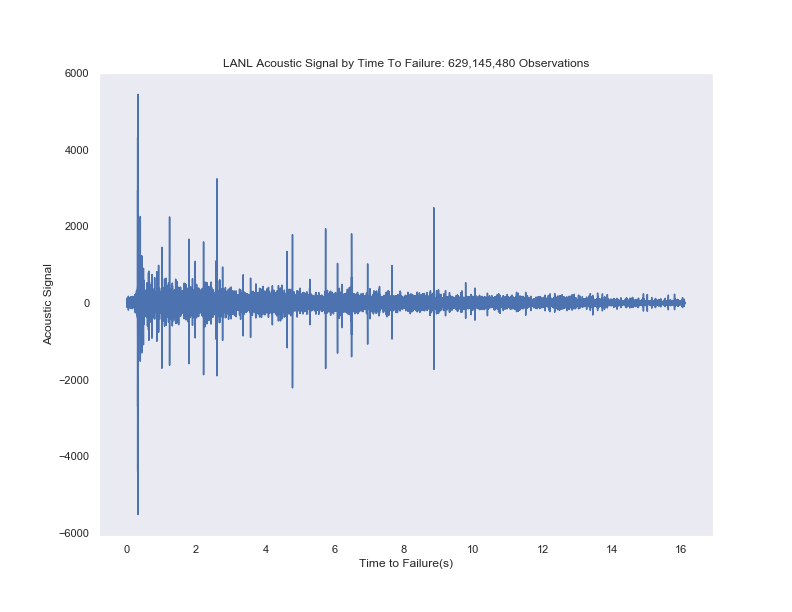
\includegraphics[width=0.7\linewidth]{../GPUProject/allDataDefaultPlot}
	\caption{The magnitude of each seismic signal and its related time remaining before the next laboratory earthquake.}
	\label{fig:alldatadefaultplot}
\end{figure}

\begin{table}[h!]
	\begin{center}
		\caption{Sample of Data Provided}
		\label{tab:table1}
		\begin{tabular}{l|c|r} % <-- Alignments: 1st column left, 2nd middle and 3rd right, with vertical lines in between
			\textbf{Index} & \textbf{Seismic Signal} & \textbf{Time to Failure}\\
			\hline
			0 & 12 & 1.469099998474121 \\ 
			1 & 6 & 1.469099998474121 \\ 
			2 & 8 & 1.469099998474121 \\ 
			3 & 5 & 1.469099998474121 \\ 
			4 & 8 & 1.469099998474121 \\ 
		\end{tabular}
	\end{center}
\end{table}

\begin{figure}
	\centering
	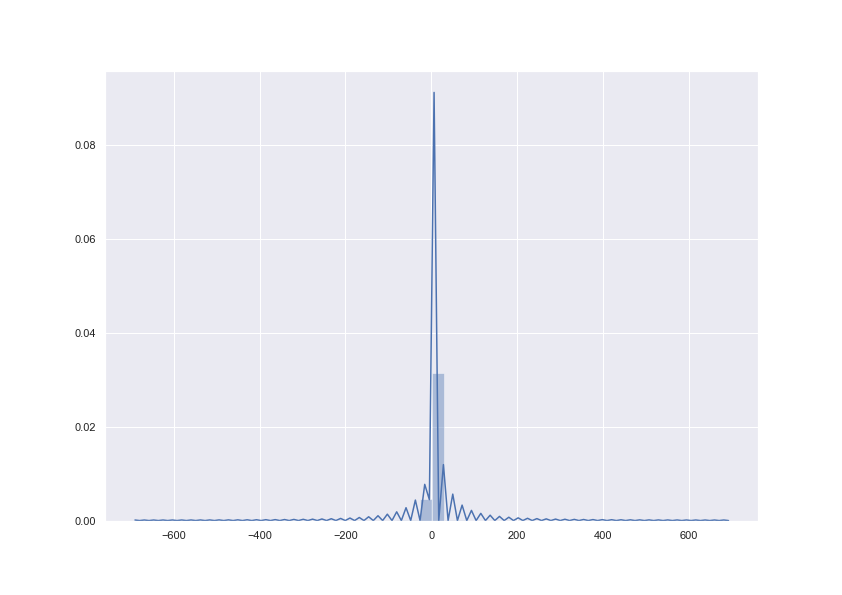
\includegraphics[width=.8\linewidth]{../GPUProject/acousticRand60000DistPlot}
	\caption{The distribution of seismic signal measurements by LANL}
	\label{fig:acousticRand60000DistPlot}
\end{figure}

The data was generated by a standard laboratory earthquake physics set-up called {\em tbd}.  
The 629,143,480 observations are a continuous segment. The seismic signals are signed integer values ranging from {\em min max}. They are acoustic and {\em hopefully we find more information about this}. The time to failure recordings are floating point decimal ranging from {\em min max} in seconds. \par

\begin{table}[h!]
	\begin{center}
		\caption{Seismic Signal Sample}
		\label{tab:table1}
		\begin{tabular}{c|c} % <-- Alignments: 1st column left, 2nd middle and 3rd right, with vertical lines in between
			\textbf{Index} & \textbf{Signal}\\
			\hline
			0 & 3 \\
			1 & 10 \\ 
			2 & 4 \\
			3 & 4 \\
			4 & 1 \\
		\end{tabular}
	\end{center}
\end{table}

\subsubsection{Kaggle Competition} Additional seismic signal data is provided with the time remaining excluded. The intention is to predict the time remaining and submit to Kaggle for scoring in the competition\cite{kaggle}. It is a collection of 2624 segments with 150,000 observations in each. The data in each segment is continuous {\em within} but {\em not} between.\par

There was one file in the test folder for each prediction (seg id) in sample submission: \par
\begin{table}[h!]
	\begin{center}
		\caption{Competition Data}
		\label{tab:table1}
		\begin{tabular}{l|c|c} % <-- Alignments: 1st column left, 2nd middle and 3rd right, with vertical lines in between
			\textbf{Index} & \textbf{Segment Id} & \textbf{Time to Failure}\\
			\hline
			0 & seg 00030f & 0 \\ 
			1 & seg 0012b5 & 0 \\ 
			2 & seg 00184e & 0 \\ 
			3 & seg 003339 & 0 \\ 
			4 & seg 0042cc & 0 \\ 
		\end{tabular}
	\end{center}
\end{table}


One huge csv file had all the training data, which is a single continuous experiment. There were only two columns in this file:
Acoustic data (int16): the seismic signal; Time to failure (float64): the time until the next laboratory earthquake (in seconds). There were no missing values for both columns. \par

\subsubsection{Acoustic Data}
The acoustic feature were integers in the range [-5515, 5444] with mean 4.52. The plot below is using a 1 percent random sample (~6M rows):
\begin{figure}[h]
	\centering
	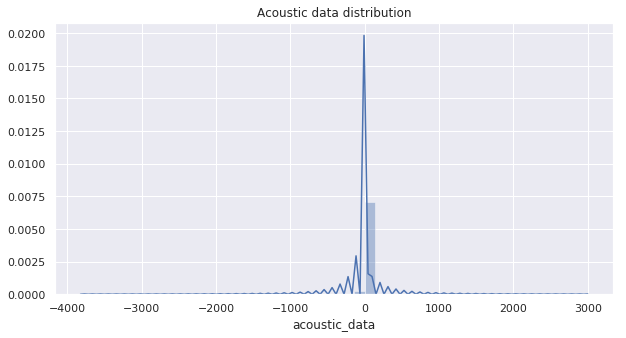
\includegraphics[width=0.7\linewidth]{../GPUProject/acousticFeatureIntegers}
	\caption[]{1\% random sample from 629,143,480 observations}
	\label{fig:acousticfeatureintegers}
\end{figure}

\subsubsection{Time to Failure}
The target variable was given in seconds:
\begin{table}[h!]
	\begin{center}
		\caption{Sample of Data Provided}
		\label{tab:table1}
		\begin{tabular}{l|c|r} % <-- Alignments: 1st column left, 2nd middle and 3rd right, with vertical lines in between
			\textbf{Index} & \textbf{Seismic Signal} & \textbf{Time to Failure}\\
			\hline
			count &  6.29145480\\ 
			mean & 4.47708428 \\ 
			std &  2.61278939\\ 
			min &  9.55039650\\ 
			25 & 2.62599707 \\ 
			50 &  5.34979773\\ 
			75 &  8.17339516\\ 
			max & 1.61074009 \\ 
		\end{tabular}
	\end{center}
\end{table}
\begin{figure}[h]
	\centering
	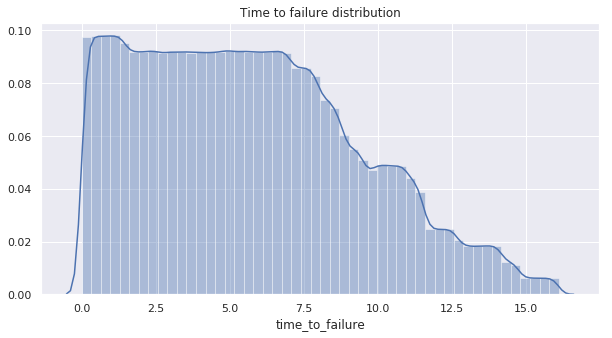
\includegraphics[width=0.7\linewidth]{../GPUProject/timeToFailureDistribution}
	\caption[]{The min value was very close to zero (around 10\^-5) and the max was 16 seconds. The distribution for the random sample}
	\label{fig:timetofailuredistribution}
\end{figure}
\subsubsection{Timeseries}
\begin{itemize}
	\item We can see that usually acoustic data shows huge fluctuations just before the failure and the nature of data is cyclical
	\item Another important point: visually failures can be predicted as cases when huge fluctuations in signal are follows by small signal values. This could be useful for predicting "time\_to\_failure" changes from 0 to high values;
\end{itemize}
\begin{figure}[h]
	\centering
	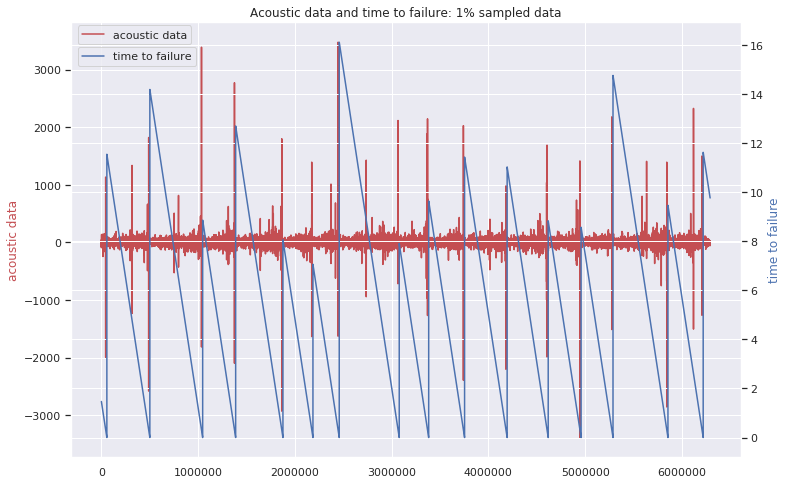
\includegraphics[width=0.8\linewidth]{../GPUProject/timeSeries}
	\caption{We checked how both variables changed over time. The red line is the acoustic data and the blue one is the time to failure. On a plot above we can see, that training data has 16 earthquakes. The shortest time to failure is 1.5 seconds for the first earthquake and 7seconds for the 7th, while the longest is around 16 seconds.}
	\label{fig:timeseries}
\end{figure}

\begin{figure}
	\centering
	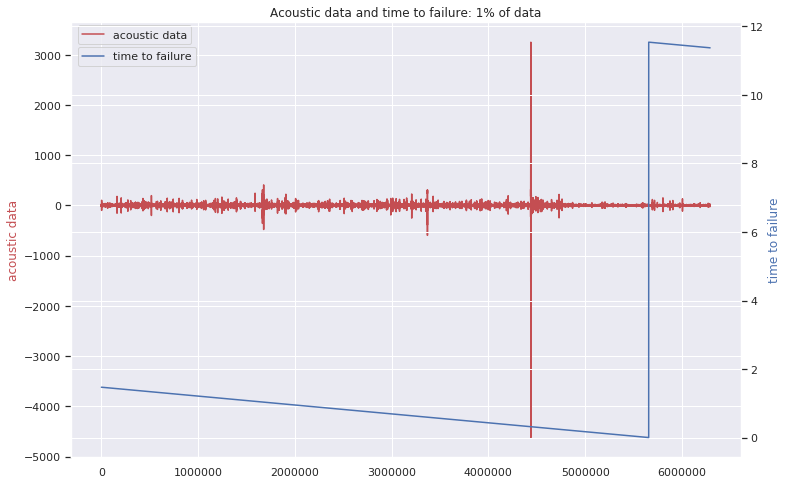
\includegraphics[width=0.7\linewidth]{../GPUProject/zoomedInTimePlot}
	\caption{On this zoomed-in-time plot we can see that actually the large oscillation before the failure is not quite in the last moment. There are also trains of intense oscillations proceeding the large one and also some oscillations with smaller peaks after the large one. Then, after some minor oscillations, the failure occurs. Interesting thing to check is the time between high levels of seismic signal and the earthquakes. We are considering any acoustic data with absolute value greater than 1000 as a high level}
	\label{fig:zoomedintimeplot}
\end{figure}
\begin{table}[h!]
	\begin{center}
		\caption{Sample of Data Provided}
		\label{tab:table1}
		\begin{tabular}{l|c|r} % <-- Alignments: 1st column left, 2nd middle and 3rd right, with vertical lines in between
			\textbf{Index} & \textbf{Seismic Signal} & \textbf{Time to Failure}\\
			\hline
			count & 11325 \\ 
			mean & 0.64454830 \\ 
			std & 1.32147193 \\ 
			min & 0.31079626 \\ 
			25 & 0.31549615 \\ 
			50 & 0.31689683 \\ 
			75 & 0.32029617 \\ 
			max & 8.86059952 \\ 
		\end{tabular}
	\end{center}
\end{table}
\begin{tabular}{|c|c|}
	
\end{tabular} 










\begin{figure}
	\centering
	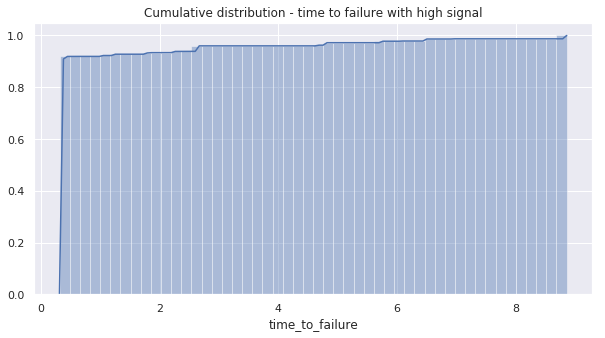
\includegraphics[width=0.7\linewidth]{../GPUProject/moreThan90percent}
	\caption{More than 90\% of high acoustic values are around 0.31 seconds before an earthquake}
		\label{fig:morethan90percent}
	\end{figure}






\section{METHODS AND EXPERIMENTS}
Describe the solution approach here.
\subsection{Data Transformations}
Explain what we did to the data here.
Explain our train and test data here.

\subsection{Recursive Neural Network}
Mean absolute = 0.5680
Patrick Yam: LSTM cannot handle data with 150000 sequence length therefore we wavenet in the earlier layers as feature extraction and reduce the sequence length to 150.\par

LSTM is a type of RNN that helps us deal with vanishing or exploding gradients (incorrect slope). For example most of our observations are within x time to failure (insert zoomedInTimePlot.png) however more extreme occur just before failure. The extreme differences in the slope difference between these observations can skew the accuracy of more traditional RNN algorithms.

LSTM separates the long term(fault slip) from short term (slow slip)
Hidden state= memory from prior observations
Typical RNN input+priorhiddenstate>tanh (-1,1) activation function>new hidden state
LSTM is same but includes gates to determine what information is included in hidden state and what is not.

The gates are rnn's themselves.

input+priorhiddenstate>sigmoid (0,1) activation function>new hidden state. 0, 1 allows us to forget or remmeber 

Forget gate decides what to include 1, or exclude 0. 
https://www.youtube.com/watch?v=2GNbIKTKCfE
https://www.youtube.com/watch?v=8HyCNIVRbSU

\subsection{Auto Regressive integrated Moving Average (ARIMA)}
The data shows evidence of non-stationarity (the mean, variance change over time). We use an ARMIA model to analyze the changing means and variance. This this model also accounts for white noise.\par ARIMA(0,0,0). Check Wikipedia.

\subsection{Gradient Boosting Decision Tree}
http://mlexplained.com/2018/01/05/lightgbm-and-xgboost-explained/
mean absolute error: 2.230923263623967
r2 score: 0.42923076680297423


%Define algorithms, methods and experiments
%DO NOT give play by play of everything we did
%Dont put code in paper; if anything put in appendix.
%Put versions of software but no one cares about how to use technology; just state what we did.
\section{RESULTS}
{\em Include evaluation methodology}
We measure this by Abolute Mean Square error

It is clear that the LSTM + Wave-net algorithms are superior performers.
This is because it handles extreme variations in the slope (gradient descent) and we can tune it to remember not only the common signals but the extreme signals which occur only when failure is imminent.
Results of experiments
Use tables and graphs
Use tables and graphs
Use tables and graphs
Don't forget explanations
\section{ANALYSIS}
Analyze results.
These are NOT conclusions.
\section{ETHICS}
If people believe us and we are wrong; bad things can happen. If people believe us and we are right; good and bad things can happen.
\section{CONCLUSION}
{\em Draw a minimum of 3 conclusions  This is NOT a summary section.} 
\par



The evidence in this new {\em observational} study suggests that {\em (Measure against prior study TBD. We have to state the fact that we cannot prove that the data collection technology improvements are better or that our algorithm is better unless we can accurately reproduce the prior model's results. Consider confounding variables such as different collection methods and unavailable details about the 2017 model.)}\par

We are able to predict with Mean absolute Error = 0.5680 however we  only know milliseconds before failure.
 Therefore practical applications may bee limited. This may prove useful but only applies to laboratory experiments. How to collect data for real world earthquakes?This could be used in industry perhaps researching materials for wallboard, machine parts.
\par

\bibliographystyle{splncs}
\bibliography{OlgaDan}
\end{document}
